\documentclass{article}
\usepackage[utf8]{inputenc}
\setlength{\parindent}{0cm}
\addtolength{\hoffset}{-2cm}
\addtolength{\textwidth}{4cm}
\usepackage[frenchb]{babel}
\usepackage[T1]{fontenc}
\usepackage[hidelinks]{hyperref}
\usepackage{graphicx}
\usepackage{afterpage}
\usepackage{minted}
\usepackage{pdflscape}

\title{Machine Gaming}
\author{Thomas Ibanez}
\makeindex


\begin{document}
\maketitle
\bigskip
\bigskip
\bigskip
\bigskip
\bigskip
\bigskip
\bigskip

\begin{center}
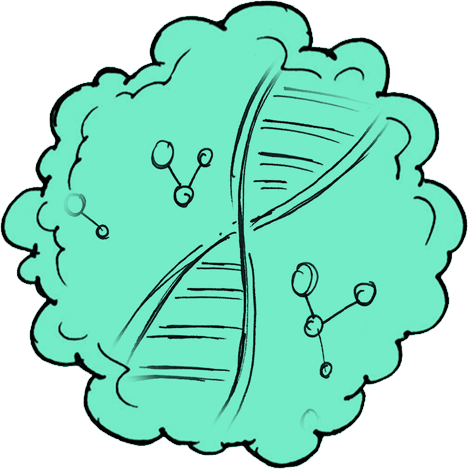
\includegraphics[scale=1]{logo.png}
\end{center}

\newpage
\tableofcontents

\newpage

\section{Introduction}

Le but de ce travail de bachelor est d'étudier et de comparer le comportement de différentes techniques de Machine Learning basés sur la neuroévolution en analysant la faculté des algorithmes à apprendre à jouer à des jeux-vidéos.\\

La neuroévolution est une technique qui constiste à faire évoluer des réseaux de neurones artificiels afin qu'ils arrivent à effectuer une tâche.\\

Un réseau de neurones est un modèle, inspiré du fonctionnement du cerveau humain, qui va consister en un ensembles de neurones artificiels (aussi appelés perceptrons), disposés en couches qui vont communiquer en propageant une information. En effet les neurones de notre cerveau vont collecter les signaux en provenance de leurs dendrites, puis si les signaux sont assez fort envoyer une impulsion le long de leur axone vers les neurones suivant qui vont faire de même. A noter que les connexions entre deux neurones peuvent être plus ou moins fortes (le signal va donc se propager avec une intensité variable).
\begin{center}
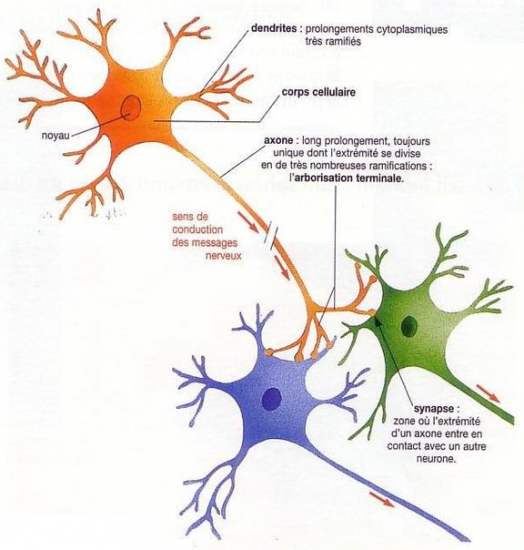
\includegraphics[scale=0.5]{neurones.png}
\end{center}

Les perceptrons quant à eux vont imiter (de manière simplifiée) ce comportement, chaque perceptron va prendre le signal envoyée par chacuns de ses voisins de la couche précédente, puis multiplier cette valeur par le poids le connexion et finalement faire le somme de toutes les valeurs pondérées et passer cette somme dans une fonction (dites fonction d'activation) qui va placer cette somme dans un interval (entre 0 et 1 par exemple) et renvoyer le resultat de cette fonction à tous ses voisins de la couche suivante qui vont faire de même.

D'un point de vue mathématique le comportement d'un perceptron peut être écrit comme:
\begin{equation}
o = f(\sum_{i=0}^{n} S_i * W_i)
\end{equation}
Où\\
$o$ est le signal qui va sortir du perceptron\\
$n$ est le nombre de voisins de la couche précédente\\
$S$ l'ensemble des signaux des voisins la couche précedente\\
$W$ l'ensemble des poids entre le perceptrons et ses voisins de la couche précédente

\begin{center}
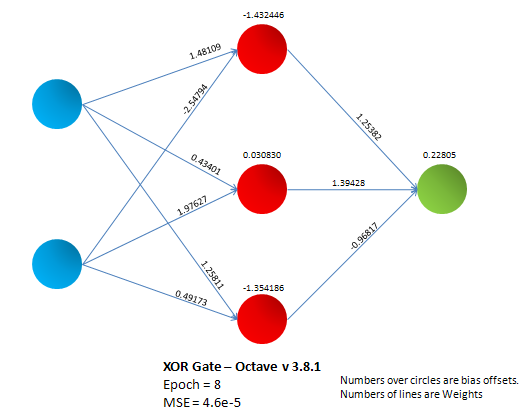
\includegraphics[scale=0.5]{XOR_Gate.png}
\end{center}

La méthode classique pour entrainer des réseaux de neurones est la rétropropagation du gradient (backpropagation). Cette technique constiste à comparer la sorties du réseaux à la sortie attendu pour une entrée donnée. L'avantage de cette technique est qu'elle va converger très rapidement vers le résultat attendu (à condition que les hyperparamètres du réseau soit adaptés au problème). Le désavantage est qu'il faut avoir à sa disposition un grand nombres d'entrées dont on connais la nature afin de pouvoir les comparer aux résultats du réseau. Par exemple il existe une base de données de chiffres écrit à la main avec leur valeur réelle sur \url{http://yann.lecun.com/exdb/mnist/} (70'000 entrées).\\

Cependant générer une telle base de données est un travail énorme, ainsi ces dernières années nous avons assisté à l'émergence de nouvelles technique ne nécessitant pas d'exemples

\section{Architecture Réseau}

Afin d'optimiser la vitesse de calcul, un système distribué à été mis en place. Celui-ci repose sur une architecture client-serveur classique où le client effectue les simulations et le serveur gère les génomes et s'occupe de distruber de manière équitable le travail entre tous les clients.\\


\subsection{Protcole}
\subsection{Serveur}
\subsection{Client}

\section{Algorithme Génétique}
\subsection{Population initiale}
\subsection{Elitisme}
\subsection{Crossover}
\subsection{Mutation}
\subsection{Génome}
\subsection{Phénome}

\section{Réseaux de Neurones}
\subsection{Perceptron Multicouche}
\subsection{NEAT}

\section{Jeux}
\subsection{Asteroid}
\subsubsection{Principe}
\subsubsection{Entrées}
\subsubsection{Sorties}
\subsubsection{Résultats}






\end{document}
